\chapter{Primer contacto con machine learning - Parte I} \label{chap:2}

\vspace*{5mm}

\section{Introducción: ¿Qué es el machine learning?} \label{sec:2.1}

El machine learning, o aprendizaje automático, es una rama de la \emph{Inteligencia Artificial} que se encarga de que los computadores aprendan a resolver problemas a partir de los datos disponibles, en lugar de programar explícitamente a la máquina para ello.

Para aprender de estos datos debemos tener claro el objetivo del problema, por ejemplo, si somos un servicio de películas online tendremos a nuestra disposición una gran cantidad de datos de nuestros clientes, tales como la lista de películas que ha visto con nosotros, sus puntuaciones, sus cuentas en redes sociales y un largo etcétera. Un problema común en este caso es saber qué películas recomendar a cierto usuario garantizando que le vaya a gustar. Así tendríamos como entrada los datos del usuario mencionados anteriormente además de una película a recomendar, $x$, y como salida si le va a gustar o no ese filme, $y$. Lo que el servicio de streaming necesita es una función ideal, casi imposible de encontrar, para predecir estas recomendaciones: $f: \mathcal{X} \rightarrow \mathcal{Y}$. Aquí $\mathcal{X}$ sería el espacio de entrada (un conjunto con todas las posibles entradas $x$), e $\mathcal{Y}$ el de salida (otro conjunto con todas las posibles salidas, en este caso \emph{sí} o \emph{no}).

No podemos olvidarnos de los datos $\mathcal{D}$, también llamados \emph{datasets} en inglés, un conjunto de relaciones entradas-salidas $(x_{1},\:y_{1}),\:\dots,\:(x_{N},\:y_{N})$, también llamadas instancias. Aquí tenemos que $y_{n} = f(x_{n})$ para $n = 1,\:\dots,\:N$, donde $N$ es el número de instancias en $\mathcal{D}$.

El problema es encontrar una función $g: \mathcal{X} \rightarrow \mathcal{Y}$ que se aproxime a $f$. Aquí interviene el aprendizaje automático, que se encarga de encontrar a $g$ en $\mathcal{H}$, un conjunto de funciones candidatas de aproximarse a $f$. Una vez que un algoritmo de machine learning es \emph{entrenado} con los datos de entrada y encuentra una $g$ que ofrezca resultados muy parecidos a los de $f$, el servicio de streaming solo deberá ofrecerle a $g$ los datos de un cliente y una pelicula a recomendar para saber si este usuario estará encantado al verla\footnote{Al proceso de usar un algoritmo una vez entrenado se le llama predecir o hacer una predicción.}. Al conjunto de posibles hipótesis $\mathcal{H}$ y al algoritmo que se utiliza se le llama \emph{modelo de aprendizaje} o simplemente \emph{modelo}.

\begin{figure}[ht]
  \centering
  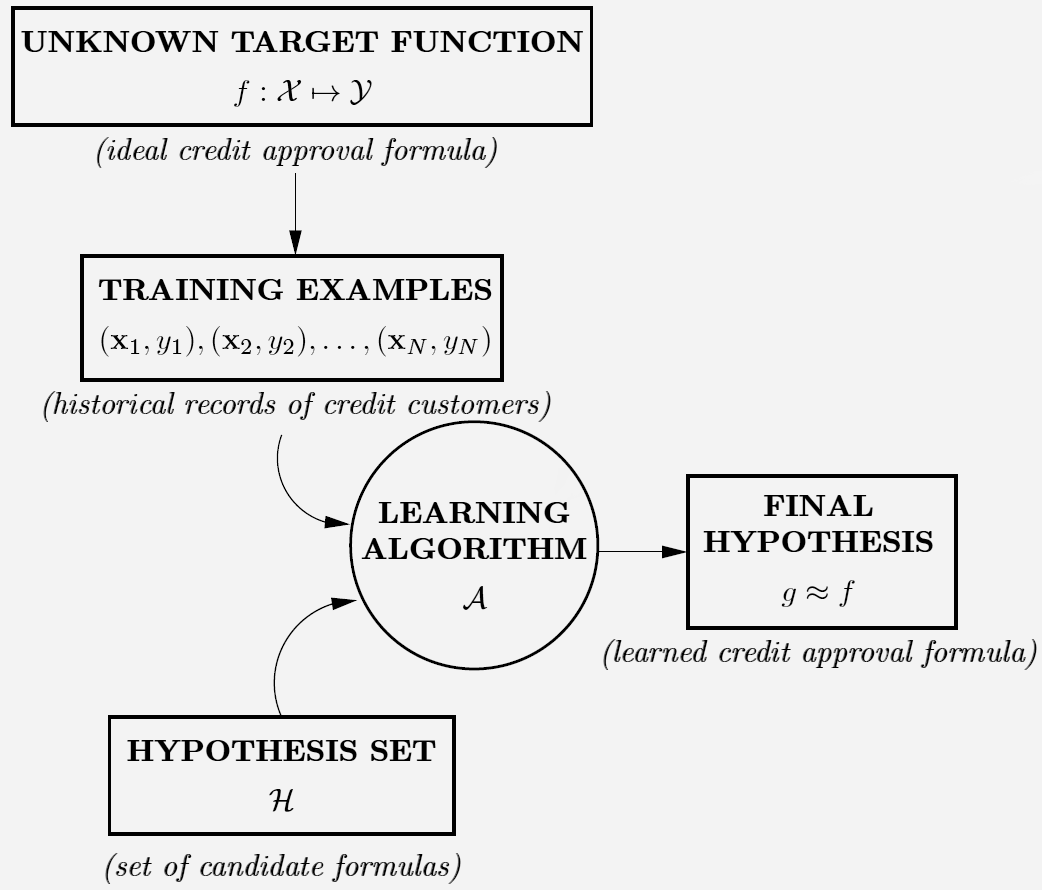
\includegraphics[width=100mm]{figures/ch_02/the_learning_problem.png}
  \caption{Disposición básica de un problema de aprendizaje. \cite{abu2012learning}}
  \label{fig:2.1}
\end{figure}

\section{Los datos y sus tipos} \label{sec:2.2}

Como vimos en la sección \ref{sec:2.1}, un dataset $D$ está formado por un conjunto instancias $(x_{n},\:y_{n})$, donde $x_{n}$ e $y_{n}$ son a su vez otro conjunto de datos, quedando entonces que $x_{n} = (x_{n,1},\:\dots,\:x_{n,M})$. Entonces, ¿qué son cada uno de los $x_{n,m}$? Si recordamos, la función $f$ tenía un espacio de entrada $\mathcal{X}$, compuesto por las variables, también llamados atributos, necesarias para poder predecir si una película gustaba a un usuario o no. Así, $x_{n,m}$ sería un valor de la variable $\mathcal{X}_{m}$, siendo $|\mathcal{X}|\:=\:M$. Aunque $|\mathcal{Y}|$ suele ser $1$, lo común si nos econtramos en otro caso suele ser transformar los datos o predecir una variable de salida a la vez.

\begin{table}[ht]
\centering
\colorbox{lightgray}{\begin{tabular}{*{5}{c}}
  $\mathbf{\mathcal{X}_{1}}$ & $\mathbf{\mathcal{X}_{2}}$ & $\mathbf{\mathcal{X}_{3}}$ & $\mathbf{\mathcal{X}_{4}}$ & $\mathbf{\dots}$ \\
  1 & 34 & H & 64 & \\
  2 & 21 & M & 130 & \\
  3 & 38 & M & 15 & \dots \\
  4 & 41 & H & 182 & \\
  5 & 25 & M & 70 & 
\end{tabular}}
\caption{Dataset de ejemplo.}
\label{table:2.1}
\end{table}

En la tabla \ref{table:2.1} podemos observar un ejemplo donde se ven algunas variables y sus valores. Estas podrían ser:

\begin{itemize}
\item[\textbullet]$\mathcal{X}_{1}$: Identificador del usuario
\item[\textbullet]$\mathcal{X}_{2}$: Edad del mismo
\item[\textbullet]$\mathcal{X}_{3}$: Sexo
\item[\textbullet]$\mathcal{X}_{4}$: Número de películas vistas por el usuario cuando se creó la instancia
\end{itemize}

Como hemos podido observar, en la tabla \ref{table:2.1} ha aparecido un valor no númerico. ¿Qué tipos de valores podemos usar con machine learning en las variables de $\mathcal{X}$ e $\mathcal{Y}$?

\begin{itemize}
\item[\textbullet]\textbf{Cuantitativos o numéricos:} Valores tanto discretos como continuos.
\item[\textbullet]\textbf{Cualitativos o categóricos:} Representan una etiqueta o categoría, como por ejemplo el sexo de una persona o si se debe o no recomendar una película a un cliente.
\end{itemize}

¿Entonces no se puede utilizar texto, imágenes o audio en los algoritmos de machine learning? La respuesta es simple, no. Pero para lidiar con esa problemática existen multitud de descriptores para aquellos tipos de información que no sean numéricos o categóricos. Estos consiguen extraer características que cumplen la restricción de que sean valores cuantitativos o cualitativos. Una selección de ellos son descritos y utilizados en \cite{richert2013building}.

\subsection{Ingeniería de atributos} \label{subsec:2.2.1}

La ingeniería de atributos es una rama del machine learning que se encarga de transformar los atributos para que estos puedan encajar en los modelos o para intentar cambiar el rendimiento de los mismos.

Existen distintas técnicas que se encargan de solucionar varios problemas, como detectar y corregir valores extremos o faltantes, corregir tipos erróneos en algunos valores de las variables o encontrar valores discriminantes que hacen que existan muy pocas instancias en algunos rangos y demasiadas en otros.

La soluciones pasan por eliminar las iteraciones problemáticas, aplicar distribuciones estadísticas o normalizar para corregir los valores. Aparte, existen algoritmos de aprendizaje que no aceptan categorías como datos de entrada. Para solucionar esto se suele usar una técnica llamada \emph{codificación de categorías}, donde las categorías son remplazadas con valores numéricos discretos, enteros, cuyos valores van desde $0$ a $|categorias| - 1$.

Además, podemos crear variables que pueden resultar muy útiles. Un ejemplo sencillo de esto puede ser el calcular el índice de masa corporal si se poseen medidas de peso y estatura, entre otras variables, para poder predecir riesgos de padecer ciertas enfermedades en datasets de pacientes. Esta nueva y simple variable puede ser muy agradecida por el rendimiento de los modelos. Aquí también se encuentran las técnicas comentadas en la sección anterior, crear descriptores para según qué tipo de información, como por ejemplo una imagen.

Una técnica que muestra una completa transformación del dataset es el \emph{bag-of-words}, técnica originada en la obtención de atributos para textos, que se ha ido exportando a otros problemas, ya que es capaz de amoldar fácilmente datasets complejos para que sean \emph{apetecibles} para los algoritmos. La primera aparición de esta técnica consistía en crear una lista con todas las palabras, o las que tuvieran un mayor valor relativo al problema, que se encontraban en el dataset, así cada instancia era otra lista de la misma longitud que la lista mencionada, conteniendo en cada posición el número de veces que esa palabra se encontraba en la instancia. 

\begin{table}[ht]
\centering
\colorbox{lightgray}{\begin{tabular}{c | c} 
  $\mathbf{\mathcal{X}_{1}}$\textbf{: Título del post} & $\mathbf{\mathcal{Y}_{1}}$\textbf{: Dificultad} \\
  Tutorial: formatear mi disco duro & Fácil \\
  Problema al formatear mi disco duro & Difícil
\end{tabular}}
\caption{Dificultad asociada a un problema según un blog de tecnología.}
\label{table:2.2}
\end{table}

\begin{table}[ht]
\centering
\colorbox{lightgray}{\begin{tabular}{*{4}{c} | c} 
  $\mathbf{\mathcal{X}_{1}}$\textbf{: tutorial} & $\mathbf{\mathcal{X}_{2}}$\textbf{: formatear} & $\mathbf{\mathcal{X}_{3}}$\textbf{: disco duro} & $\mathbf{\mathcal{X}_{4}}$\textbf{: problema} & $\mathbf{\mathcal{Y}_{1}}$\textbf{: Dificultad} \\
  1 & 1 & 1 & 0 & Fáicl \\
  0 & 1 & 1 & 1 & Difícil
\end{tabular}}
\caption{Una representación bag-of-words de la tabla \ref{table:2.2}.}
\label{table:2.3}
\end{table}

En la tabla \ref{table:2.2} vemos un pequeño dataset y en la tabla \ref{table:2.3} está una posible conversión a bag-of-words.

En el siguiente capítulo completaremos esta sección estudiando técnicas para eliminar variables, una forma de \emph{reducir la dimensionalidad} del dataset que puede mejorar el rendimiento además de la velocidad de entrenamiento y de predicción del modelo.

\section{Tipos de aprendizaje} \label{sec:2.3}

Al ser aprendizaje automático una técnica basada en aprendizaje a partir de datos, hay que dividir el tipo de aprendizaje según la naturaleza de estos datos. Detallaremos los más importantes y comentaremos algunos más, pero existen y existirán cada vez más, debido a la cambiante naturaleza de los datos.

\subsection{Aprendizaje supervisado} \label{subsec:2.3.1}

Llamamos aprendizaje supervisado a aquel cuyo datos usados para el entrenamiento poseen explícitamente en la salida las clases o categorías que el algoritmo debe producir. Es el tipo que hemos visto hasta ahora con el ejemplo de las recomendaciones de películas, donde la salida sería \emph{sí} o \emph{no}.

Este tipo de aprendizaje es el más común, dado por la topología de los datos, ya que lo normal es disponer de alguna clasificación implícita en algunas de sus variables.

\subsection{Aprendizaje por refuerzo} \label{subsec:2.3.2}

Cuando el conjunto de datos no indica explícitamente la salida correcta para una instancia dejamos de estar en aprendizaje supervisado, donde las instancias tenían la forma $(entrada,\:salida\:correcta)$. En el \emph{aprendizaje por refuerzo} disponemos en cada instancia de una salida que produce la entrada y de una medida de cómo de buena es la salida, algo como $(entrada,\;salida,\;grado\;para\;esta\;salida)$.

\begin{table}[ht]
\centering
\colorbox{lightgray}{\begin{tabular}{*{2}{c} | *{2}{c}} 
  $\mathbf{\mathcal{X}_{1}}$\textbf{: Estado} & $\mathbf{\mathcal{X}_{2}}$\textbf{: Jugada} & $\mathbf{\mathcal{Y}_{1}}$\textbf{: Estado} & $\mathbf{\mathcal{Y}_{2}}$\textbf{: Grado} \\
  $E_{i}$ & $B2 \rightarrow C3$ & $E_{j}$ & 0.35 \\
  $E_{n}$ & $D4 \rightarrow C5$ & $E_{m}$ & 0.90
\end{tabular}}
\caption{Dos muestras de un ficticio dataset de jugadas de damas.}
\label{table:2.4}
\end{table}

Por ejemplo, en la tabla \ref{table:2.4} vemos dos muestras de un dataset para un juego de mesa como las damas, donde podemos realizar diferentes acciones, no existiendo ninguna $100\%$ correcta. Aquí tendríamos como datos de entrada el estado de la partida y el movimiento a realizar, por lo que como salida tendríamos un nuevo estado y una medida de cómo le fue de bien a largo plazo al jugador, representado por $0.0$, la peor jugada posible; $1.0$, la mejor; y sus valores intermedios.

\subsection{Aprendizaje no supervisado} \label{subsec:2.3.3}

En el \emph{aprendizaje no supervisado} no disponemos de ninguna salida en el conjunto de datos, $|\mathcal{Y}|\:=\:0$, tan solo tenemos datos de entrada, $|\mathcal{X}|\:\geq\:1$. Nos podemos preguntar cómo podemos aprender de unos datos así, pero para ello tenemos que conocer cómo funcionan los problemas de \emph{agrupamiento} en machine learning, cosa que veremos en la sección \ref{sec:2.4} (\emph{\nameref{sec:2.4}}). Para hacer un adelanto, se puede pensar en problemas donde se tienen que clasificar libros por su temática sin conocerla previamente, solo fijándonos en propiedades similares que estos tengan para agruparlos en una categoría.

Este tipo de aprendizaje tiene una característica muy importante, puede descubrir patrones que eran desconocidos en los datos. Esto ocurre al no tener una definición previa, la salida, de lo que se quiere obtener.

\subsection{Otros tipos de aprendizaje} \label{subsec:2.3.4}

También podemos clasificar el aprendizaje según la forma de obtención de los datos, ya que lo común es tener todo el conjunto de datos listo antes de comenzar con el aprendizaje, aunque eso no siempre puede ser posible. Por ejemplo, existe un subtipo llamado \emph{aprendizaje activo}, donde el dataset es adquirido por medio de consultas.

Por otro lado, si el conjunto de datos se va incrementado en una instancia cada vez, por ejemplo, en mediciones de sensores, el aprendizaje pasaría a llamarse \emph{aprendizaje en línea}.

\section{Tipos de problemas} \label{sec:2.4}

Los datos en un caso práctico de machine learning no solo afectan al tipo de aprendizaje que se pueda realizar, sino también al tipo de problema a resolver, y por ende al modelo que se pueda usar. Veamos los principales tipos de problemas, para más tarde, en la secciones \ref{sec:2.5} y \ref{sec:3.1}, ver distintos tipos de algoritmos para cada uno. 

\subsection{Agrupamiento} \label{subsec:2.4.1}

Como vimos en la subsección \ref{subsec:2.3.3} (\emph{\nameref{subsec:2.3.3}}), el agrupamiento, \emph{clustering} en inglés, consiste en \emph{clasificar} sin usar la salida, sino fijándose en la \emph{similaridad} de las variables de entrada de cada instancia. Dependiendo del algoritmo de agrupamiento utilizado, esa similaridad será distinta. Una vez que el algoritmo haya finalizado su aprendizaje, tendremos las instancias agrupadas en distintos \emph{clusters}, donde cada elemento dentro de cada cluster será similar a los demás de ese mismo grupo. En la figura \ref{fig:2.2} tenemos un ejemplo donde cada cluster tiene un color distinto.

\begin{figure}[ht]
  \centering
  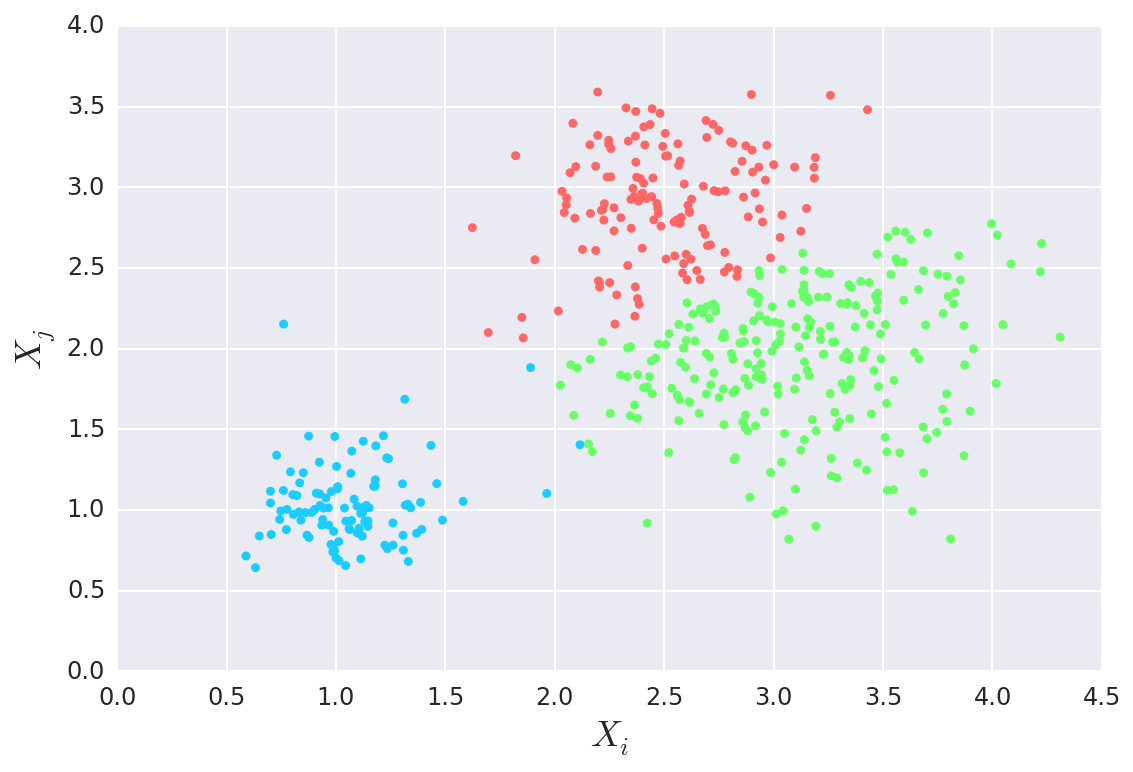
\includegraphics[width=100mm]{figures/ch_02/clustering_example.png}
  \caption{Representación visual de un ejemplo de agrupamiento, donde se agrupan dos variables de entrada, $\mathcal{X}_{i}$ y $\mathcal{X}_{j}$, dando lugar a tres grupos representados por colores diferentes.}
  \label{fig:2.2}
\end{figure}

En la subsección \ref{subsec:2.5.1} veremos las \emph{\nameref{subsec:2.5.1}}, uno de los algoritmos de agrupamiento, que puede devolver un agrupamiento como el de la figura \ref{fig:2.2} 

\subsection{Clasificación} \label{subsec:2.4.2}

La clasificación es el problema más común a resolver en el aprendizaje supervisado (subsección \ref{subsec:2.3.1}). El nombre de este tipo de problemas viene dado por su objetivo, separar las instancias de $\mathcal{D}$ en diferentes \emph{clases} según sus atributos.

Existen subtipos dentro de éste, como la clasificación binaria, donde solo existen dos clases a aprender; la clasificación multiclase, donde existen más dos clases en las que clasificar las instancias; y la clasificación multicategórica, donde las instancias pueden tener como salida más de una clase. Dependiendo de este subtipo hay que ajustar los algoritmos, o usar otros distintos.

Los algoritmos de clasificación que veremos en este texto son:

\begin{itemize}
\item[\textbullet]\nameref{subsec:2.5.2}, subsección \ref{subsec:2.5.2}
\item[\textbullet]\nameref{subsec:2.5.3}, subsección \ref{subsec:2.5.3}
\item[\textbullet]\nameref{subsec:2.5.4}, subsección \ref{subsec:2.5.4}
\item[\textbullet]\nameref{subsec:3.1.1}, subsección \ref{subsec:3.1.1}
\item[\textbullet]\nameref{subsec:3.1.2}, subsección \ref{subsec:3.1.2}
\item[\textbullet]\nameref{subsec:3.1.3}, subsección \ref{subsec:3.1.3}
\end{itemize}

\subsection{Regresión} \label{subsec:2.4.3}

Similar a la \emph{clasificación \textbf{no} multicategórica} (subsección \ref{subsec:2.4.2}), la regresión solo tiene una variable de salida, y además es numérica y continua. Estos problemas enmascaran una manera imposible de trabajar para los clasificadores\footnote{Clasificadores: nombre que reciben los algoritmos que resuelven problemas de clasificación.}, hacer clasificación multiclase con infinitas clases.

Los algoritmos que pueden resolver problemas de regresión son los mismos que los de clasificación (subsección \ref{subsec:2.4.1}), solo tienen que usar pequeñas modificaciones antes de devolver su salida, salvo la mayoría de regresiones (subsección \ref{subsec:3.1.1}), cuyo uso original es para regresión.

\section{Algoritmos - Parte I} \label{sec:2.5}

Hasta aquí se han visto algunas ideas generales sobre machine learning que hacen que ya se tengan ciertas ideas correctas en la cabeza, como por ejemplo cómo funciona a muy grandes rasgos un algoritmo de aprendizaje y cuáles son los datos de los que se puede alimentar.

A continuación estudiaremos cuatro de los principales algoritmos del aprendizaje automático, continuando con algunos más en el capítulo \ref{chap:3}.

\subsection{$k$-medias} \label{subsec:2.5.1}

El primero de los algoritmos, $k$-medias, usa aprendizaje no supervisado para resolver un problema de clustering, devolviendo el punto medio de cada cluster. Usando este procedimiento, encontraremos una función $g$ que utilizando el conjunto de datos $\mathcal{D}$ y un entero $k$, devolverá $k$ clusters, siendo $k$ una variable que tenemos que definir. Hay métodos heurísticos para definir la mejor $k$ para cada problema, ya que su elección dictamina claramente el resultado del algoritmo. Veamos el pseudocódigo de este algoritmo para posteriormente ampliar varias de sus partes:

\vspace*{3mm}
\lstset{style=pseudocode}
\begin{lstlisting}
definir $k$-medias($Y_{t}$, $Y_{t\:-\:1}$, $u$):
  calcular distancias entre $Y_{t}$ e $Y_{t\:-\:1}$
  si distancias menores que $u$:
    para cada $x_{i}$ en $\mathcal{D}$:
      calcular distancia a cada $y_{t,\:i}$
      asociar $x_{i}$ a $y_{t,\:i}$ mas cercano
    para cada $y_{t,\:i}$:
      calcular centroide como $y_{t\:+\:1,\:i}$ de cada $x_{i}$ asociado a $y_{i,\:i}$
    $k$-medias($Y_{t\:+\:1}$, $Y_{t}$)
  si no:
    devolver $Y_{t}$

crear $k$ puntos_de_control de dimension $|\mathcal{X}|$
crear $k$ puntos_en_el_infinito de dimension $|\mathcal{X}|$
$k$-medias(puntos_de_control, puntos_en_el_infinito, umbral)
\end{lstlisting}

Aquí vemos cómo el primer paso es crear $k$ puntos de control, $Y\:=\:(y_{1},\:...,\:y_{k})$, de dimensión $|\mathcal{X}|$, la del espacio de entrada. Esto se puede realizar de forma aleatoria, pero existen métodos para calcular $k$ puntos dado $\mathcal{D}$ que consiguen agilizar y casi asegurar la convergencia del algoritmo.

Al calcular la distancia entre cada punto $x_{i}$ en $\mathcal{D}$ y todos los puntos en $Y_{t}$ y asociarlos a los $y_{t,\:i}$ más cercanos se consiguen crear grupos temporales, que pueden ser los definitivos si se trata de la ultima recursión. Para calcular esta distancia normalmente se usa la distancia euclidea\footnote{Euclidean distance, entrada en Wikipedia: \url{http://en.wikipedia.org/wiki/Euclidean_distance}}, aunque por supuesto se pueden usar otras:

$$
d(x_{i},\:y_{t,\:i})\:=\:\sqrt{\sum_{j\:=\:1}^{|\mathcal{X}|}(x_{i,\:j}\:-\:y_{t\:i,\:j})^{2}}
$$

\noindent
donde $j$ indica la posición $j$-ésima de cada varaible en $x_{i}$ e $y_{t,\:i}$.

Para calcular los centroides y obtener los nuevos $y_{t\:+\:1,\:i}$ simplemente se usa la media aritmética de cada $x_{i}$ asociado a $y_{t,\:i}$, tratando dichos $x_{i}$ no como valores individuales, sino como los vectores que son, siendo sus elementos valores de las variables de $\mathcal{X}$:

$$
y_{t\:+\:1,\:i}\:=\:\frac{\sum_{i\:=\:1}^{N}x_{i}}{N}
$$

\noindent
donde $N$ es el número de $x_{i}$ asociados a $y_{t,\:i}$.

Para finalizar el análisis del algoritmo podemos observar que la condición de parada del algoritmo es que todos los puntos de $Y_{t}$ actuales estén a una distancia menor que el umbral, $u$, respecto a los puntos de la recursión anterior, $Y_{t\:-\:1}$:

$$
\forall\:y_{t,\:i}\:\backslash\:d(y_{t,\:i},\:y_{t\:-\:1,\:i}) < u
$$

\noindent
observando así que para el primer paso es buena idea colocar los puntos previos, $Y_{t-1}$, en el infinito.

\begin{figure}[ht]
  \centering
  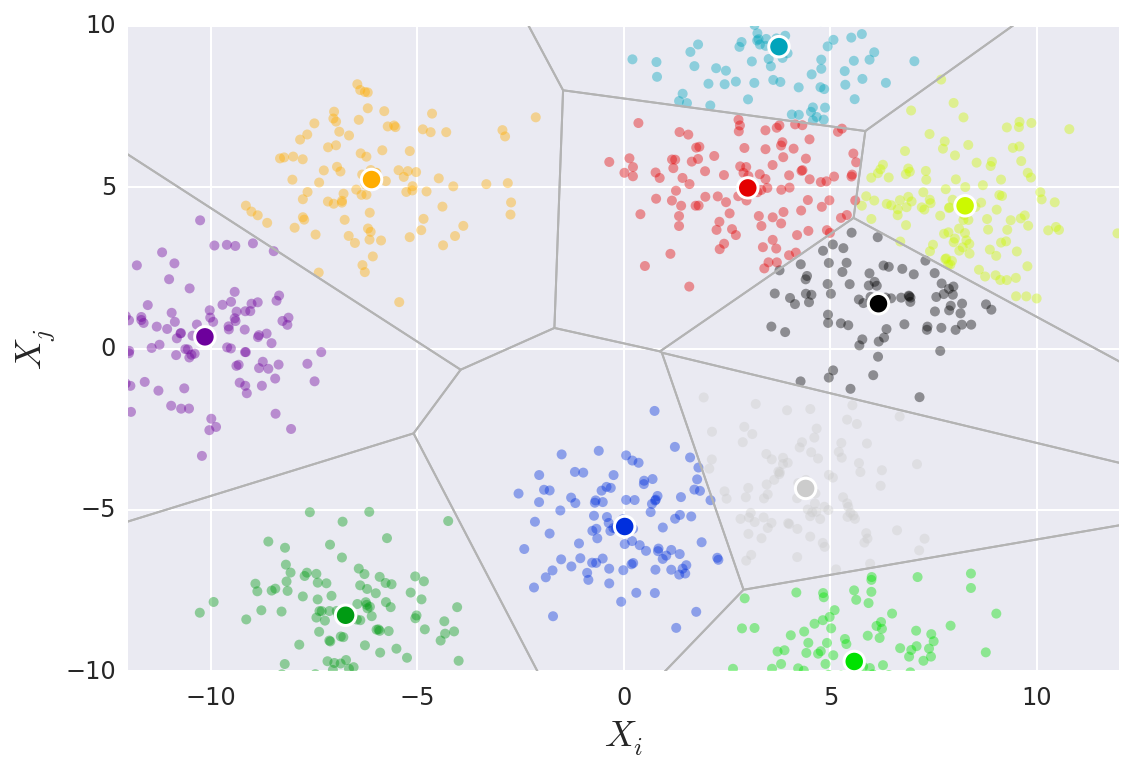
\includegraphics[width=100mm]{figures/ch_02/kmeans_example.png}
  \caption{Representación de un resultado obtenido por $k$-medias.}
  \label{fig:2.3}
\end{figure}

En la figura \ref{fig:2.3} podemos ver la representación gráfica del resultado que puede ofrecer un ejemplo del algoritmo $k$-medias cuando los datos tienen como dimensionalidad $\mathcal{X} = 2$. Además, se han dibujado los centroides y las líneas limítrofes de cada cluster. En resumen, este algoritmo crea ciertos puntos y los va moviendo por los valores de $\mathcal{X}$ hasta que la distancia entre movimientos sea mínima.

\subsection{$k$-NN} \label{subsec:2.5.2}

El algoritmo de los $k$-vecinos más cercanos, \emph{$k$-nearest neighbors} en inglés, puede ser el más \emph{simple} de todos, teniendo mejor rendimiento en su resultado que muchos métodos más complejos. Además no requiere entrenamiento, directamente es capaz de predecir.

\vspace*{3mm}
\lstset{style=pseudocode}
\begin{lstlisting}
definir $k$-NN($\mathcal{D}$, $x_{pred}$):
  crear $salida$ como conjunto ordenado vacio
  para cada $x_{i}$ en $\mathcal{D}$:
    calcular distancia entre $x_{pred}$ y $x_{i}$
    introducir $x_{i}$ en $salida$ en orden segun distancia
  devolver los $k$ elementos de $salida$ con menor distancia

$k$-NN($\mathcal{D}$, $x_{pred}$)
\end{lstlisting}

Como se ve en el pseudocódigo anterior, $k$-NN calcula las $k$ instancias más cercanas a la que quiere predecir, $x_{pred}$, utilizando la distancia que se desee, normalmente la euclídea como se vio en la subsección de las \nameref{subsec:2.5.1}. Esto hace que sea unos de los algoritmos con peor rendimiento computacional a la hora de predecir, ya que tiene que recorrer todas las instancias para calcular las distancias, aunque existen métodos de búsqueda para mejorar este problema.

Tras encontrar a los $k$-vecinos más cercanos se crea la predicción. Si estamos ante un problema de clasificación el algoritmo tiene que escoger una clase de todas la resultantes, siendo lo más común escoger la clase que más se repita, incluso se puede apoyar en ponderar el resultado según la distribución de las clases en las instancias. Si estamos en un problema de regresión, lo usual es hacer la media aritmética de los resultados o una media ponderada a una distribución como en el caso de la clasificación.

$$
\bar{x}\:=\:\frac{\sum_{i\:=\:1}^{k}x_{i}\:w_{i}}{\sum_{i\:=\:1}^{k}w_{i}}
$$

Como se observa, la media ponderada hace que cada valor $x_i$ que se use para el resultado, tenga un peso asociado $w_{i}$.

\subsection{Regresión lineal} \label{subsec:2.5.3}

La regresión lineal es un método que predice valores reales, no clasificaciones, como vimos en la subsección \ref{subsec:2.4.3}, aunque como se comentó anteriormente es posible transformarlo para clasificar. El concepto más importante de esta solución es el mismo que el de la recta de mínimos cuadrados. Nuestra función $g$ será, de entre todas las hipótesis en $\mathcal{H}$, una recta que minimice el error cuadrático\footnote{En la subsección \emph{\ref{subsec:3.2.3} \nameref{subsec:3.2.3}} se estudia la medida del error.} respecto a $f$\footnote{Recordar que $f$ era la función ideal que se busca en problemas de machine learning}, como el ejemplo que se muestra en la figura \ref{fig:2.4}.

Cuando hablamos de una recta, significa que nuestro problema solo tiene dos dimensiones, una en $\mathcal{X}$ y otra en $\mathcal{Y}$. Conforme aumenta la dimensionalidad del problema, también aumentan el número de variables en el espacio de entrada $\mathcal{X}$ y dejamos de buscar un recta para buscar su generalización, el \emph{hiperplano}. Por ejemplo, si tenemos que $|\mathcal{X}|\:=\:2$, tenemos un problema de tres dimensiones y nos encontraríamos en el caso de buscar el plano de los mínimos cuadrados.

\begin{figure}[ht]
  \centering
  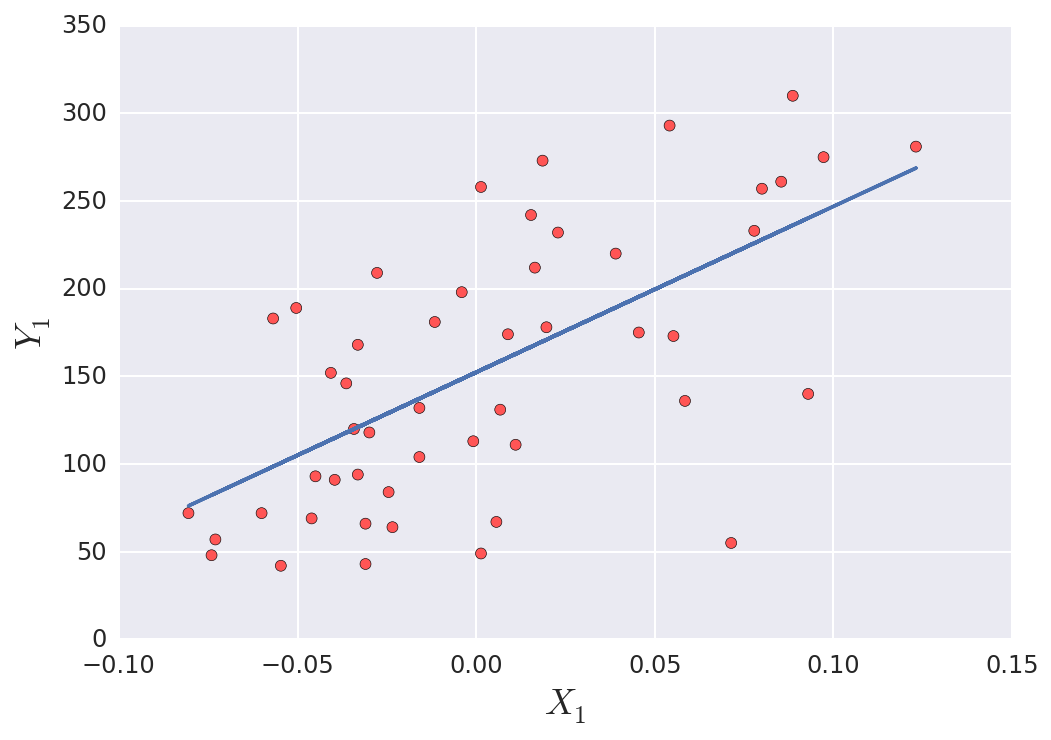
\includegraphics[width=100mm]{figures/ch_02/regression_example.png}
  \caption{Representación de una regresión lineal, además de ser una recta de mínimos cuadrados.}
  \label{fig:2.4}
\end{figure}

Veamos los pasos necesarios para construir la función $g$ para cualquier dimensión. Se ofrece un punto de vista más matemático y algo menos algorítmico que las $k$-medias, ya que durante el proceso se trabaja con \emph{matrices} y se trata de ofrecer una fácil representación del proceso:

\noindent\colorbox{lightgray}{
\begin{minipage}{\dimexpr\textwidth-2\fboxsep}
\begin{enumerate}
\item Construir la matriz $A$ y el vector $\textbf{y}$ a partir de las instancias del dataset $\emph{D}$, $(x_{1},\:y_{1}),\:\dots,\:(x_{N},\:y_{N})$, donde a cada $x_{i}$ se le incluye un elemento $x_{i,\:0}\:=\:1$, que se convertirá en un término independiente en la función:

$$
A\:=\:\begin{bmatrix}
x_{1} \\
x_{2} \\
\vdots \\
x_{N}
\end{bmatrix},
\hspace{15mm}
\textbf{y}\:=\:\begin{bmatrix}
y_{1} \\
y_{2} \\
\vdots \\
y_{N}
\end{bmatrix}
$$

\item Calcular $A^{+}$, la matriz pseudoinversa de $A$. Si la matrix $A^{T}A$ posee inversa, se puede usar el siguiente método:

$$
A^{+}\:=\:(A^{T}A)^{-1}A^{T}
$$

\item Crear $w\:=\:A^{+}\textbf{y}$

\item Devolver la función

$$
g(x_{i})\:=\:w_{0}\:+\:\:x_{i,\:1}w_{1}\:+\:x_{i,\:2}w_{2}\:+\dots\:+\:x_{i,\:M}w_{M}
$$
\centerline{Siendo $M\:=\:|\mathcal{X}|\:\:\:\:\:\:\:\:\:\:\:\:\:\:\:\:\:\:\:$}

\end{enumerate}
\end{minipage}
}

\vspace*{3mm}

En el caso de que tuviéramos dimensión 2, una variable en $\mathcal{X}$ y otra en $\mathcal{Y}$, la ecuación devuelta sería la recta de mínimos cuadrados:

$$
g(x_{i})\:=\:w_{0}\:+\:\:x_{i,\:1}w_{1}
$$

\noindent
que se puede denotar como la ecuación de la recta:

$$
y\:=\:ax\:+\:b
$$

\noindent
donde ofreciendo la entrada que queremos predecir, $x$, nos devuelve la predicción $y$.

Los algoritmos de este tipo\footnote{Existe más regresiones muy usadas, como la \emph{regresión logística}.} son un caso extraño, ya que devuelven una ecuación que es fácil y muy rápida de evaluar, conviertiéndolos en unos regresores y clasificadores instantáneos.

\subsection{Naive Bayes} \label{subsec:2.5.4}

Naive Bayes es un algoritmo clasificador, aunque ajustándolo también puede funcionar como regresor, que utiliza la \emph{probabilidad} para ofrecer sus resultados. Veamos cómo funciona este sencillo algoritmo, aunque no podemos hacerlo paso por paso, ya que primero debemos conocer los simples pero potentes métodos que utiliza.

Simplemente, naive Bayes calcula la probabilidad de todos los posibles valores de la variable de salida, partiendo de un valor para cada variable de entrada\footnote{Esta probabilidad se llama probabilidad condicionada, $P(A|B)$, que se lee probabilidad de que ocurra $A$ sabiendo que ocurre $B$.}, y se queda con la que tenga el máximo valor:

$$
g(x_{i})\:=\:\max_{\forall\:y_{j}\:\in\:\mathcal{Y}}\:P(y_{j}|x_{i,\:1},\:x_{i,\:2},\:\dots,\:x_{i,\:n}):
$$

Esta simple probabilidad se vuelve imposible de calcular para un número grande de variables de entrada, o si éstas toman muchos valores distintos. Pero si se utiliza el \emph{teorema de Bayes}:

$$
P(A|B)\:=\:\frac{P(B|A)P(A)}{P(B)}
$$

\noindent
nuestra función $g$ quedaría como:

$$
g(x_{i})\:=\:\max_{\forall\:y_{j}\:\in\:\mathcal{Y}}\:\frac{P(x_{i,\:1},\:x_{i,\:2},\:\dots,\:x_{i,\:n}|y_{j})P(y_{j})}{P(x_{i,\:1},\:x_{i,\:2},\:\dots,\:x_{i,\:n})}
$$

\noindent
y al tener todas las posibles funciones $g(x_{i})$ el mismo denominador, se puede eliminar, quedando como:

$$
g(x_{i})\:=\:\max_{\forall\:y_{j}\:\in\:\mathcal{Y}}\:P(x_{i,\:1},\:x_{i,\:2},\:\dots,\:x_{i,\:n}|y_{j})P(y_{j})
$$

Esta función de probabilidad máxima es más simple de calcular, pero solo de manera correcta si tuviéramos una cantidad inmensa de datos. En el caso de que todas la variables de entrada sean independientes\footnote{En estadística, dos variables son independientes si la ocurrencia de una no tiene que ver con la ocurrencia de la otra.} este problema no existiría.

La parte \emph{naive} del método simplifica este problema asumiendo que todas las variables de entrada son independientes, contando con un pequeño pero despreciable error, así podemos calcular la probabilidad condicionada de $x_{i,\:j}$ respecto a $y_{i}$ de forma independiente:

$$
g(x_{i})\:=\:\max_{\forall\:y_{j}\:\in\:\mathcal{Y}}\:P(y_{j})\prod_{i\:=\:1}^{|\mathcal{X}|}P(x_{i,\:j}|y_{j})
$$

\noindent
una probabilidad fácil de resolver, y rápida, si realizamos un análisis de frecuencias previo en los datos.

\section{Continuación} \label{sec:2.6}

En el siguiente capítulo (\emph{\ref{chap:3}. \nameref{chap:3}}), continuaremos estudiando algoritmos de aprendizaje, además de algunos conceptos más para poder empezar a trabajar con machine learning, finalizando así la sección teórica del documento.
